\subsection{Tachometer} \label{sub:systemarkitektur_tachometer}

For at måle hastigheden af bilen, er det nødvendigt at designe en form for tachometer. Kravene til komponenten er at det skal være kompakt, være strømbesparende og være inden for rimelige grænser prismæssigt. Da DC-motoren som driver bilen er præfabrikeret, og der er gearing før momentet når til hjulene, bliver det hurtigt besværligt at skulle konstruere noget inde ved motoren. Alternativt er der plads ved bilens baghjul, hvilket der vælges at gå frem efter. Gruppen forslog tre muligheder, hvoraf en blev valgt til design/realiseringsfasen.

Her ses de 3 foreslåede muligheder:

\begin{enumerate}
	\item Lys-modtager/sender, som, via en skive med et prædefineret antal huller, kan detektere lys sendt fra senderen ind på skiven og detektere lyset, når det kommer igennem et af hullerne. Derved vil der kunne omregnes fra hvert hul detekteres til en konkret hastighed.
	\item Induktiv føler, som via nogle metalstykker monteret på indersiden af hjulet og en føler skulle detektere en ændring i magnetfelt, når metalstykkerne passerede føleren. På samme måde kunne dette omregnes til en konkret hastighed.
	\item Hall-switch/Reed rør, der fungerer på tilnærmelsesvist samme måde som den induktive føler, men med små magneter monteret på indersiden af hjulet. 
\end{enumerate}

Gruppen valgte at fortsætte med metode 3 - Hall-switch af typen TLE4905L \cite{lib:TLE4905L}. 

En Hall switch kan detektere ændring i magnetfelt og via en schmittrigger trækker den signalet til ground, når der er en magnet tilstede og en høj puls hvis der ikke er. På bilens hjul er fem akser, som er ligeligt fordelt over hjulets omkreds. Ved at montere en magnet på hver af akserne, kan der opnås en stor mængde data, som kan omregnes til en hastighed. 

\begin{figure}[h]
\centering
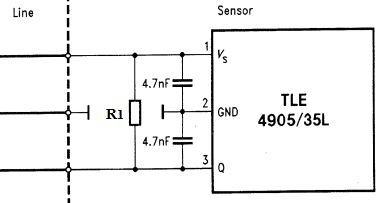
\includegraphics[scale=1]{../fig/billeder/tle4905L_application_circuit.png}
\caption{Anbefalet applikations kredsløb for TLE4905L}
\label{fig:tle4905L_app_circuit}
\end{figure}

På figur \ref{fig:tle4905L_app_circuit} ses det anbefalede applikations kredsløb for hall-switchen. I databladet kan aflæses at forsyningsstrøm ligger mellem 4mA og 8mA, da vi ønsker at trække strømmen fra et batteri, forsøges det at lægge strømmen så lavt som muligt - 4mA. Via ohms lov kan vi udregne R1 til at give ca. $1.2k\Omega$

\begin{equation}
R1 = \dfrac{5V}{4mA} = 1.25\cdot 10^3 \Omega
\end{equation}

Derved kan vi sætte $R1 = 1.25k\Omega \approx 1.2k\Omega$

TLE4905L forventes at blive monteret på bilens højre baghjul, på en måde, så kredsløbet ikke bliver forstyrret for meget af rystelser osv. 